\NoBgThispage
\section{Struttura Generale dell'Applicazione}
L’applicazione è stata sviluppata seguendo l’architettura \texttt{MVC (Model-View-Controller)}, dove le parti View e Controller sono inglobati nella User Interface (UI).
Di conseguenza il codice sorgente del package \texttt{src} è suddiviso in due Macro-package: \texttt{Models} in cui sono presenti tutte le classi che gestiscono i dati,
mentre nel package \texttt{GUI} sono presenti le classi che gestiscono la UI e l’interazione tra i comandi fatti dall’utente e lo storage dei dati.
È presente anche un package, \texttt{utils}, che contiene classi di utilità usate nella maggior parte delle altre classi.


\begin{figure}[H]
    \centering
    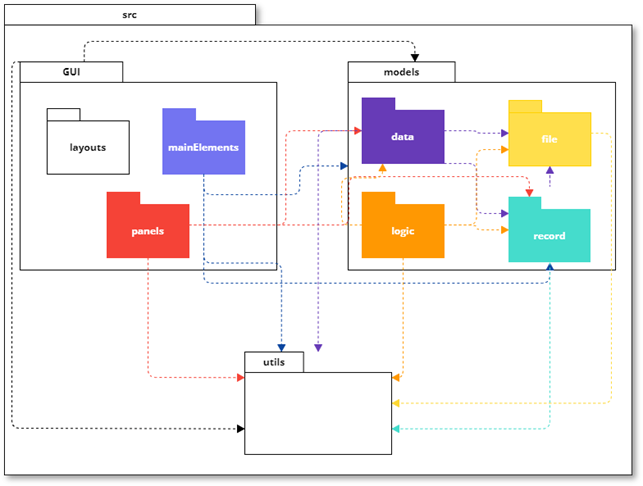
\includegraphics[width=0.7\textwidth]{../../img/package_structure.png}
    \caption{Struttura dei package dell'applicazione.}
\end{figure}